\documentclass[12pt]{article}

\title{Data Analysis Project Report}
\author{James Hughes}

\usepackage[nottoc,numbib]{tocbibind}
\usepackage{graphicx}
\usepackage[export]{adjustbox}
\usepackage[a4paper, top=13mm, bottom=19mm]{geometry}


\newcommand\NA{\mathit{NA}}

\begin{document}

\begin{titlepage}
    \begin{center}
        \vspace*{5cm}

        \Huge
        \textbf{Structured Illumination Microscopy Image Processing using Deep Learning}

        \vspace{0.5cm}
        \LARGE

        James Hughes

        Supervised by Dr Edward Ward

        \vspace{2cm}
        \Huge
        \textbf{Project Report}

        \vfill

        MPhil, Data Intensive Science

        \vspace{0.8cm}

        \Large
        Department of Physics \& Department of Chemical Engineering and Biotechnology

        University of Cambridge

        United Kingdom

        28th June 2024

    \end{center}
\end{titlepage}

\pagenumbering{roman}

\newpage
\section*{Acknowledgements}
\addcontentsline{toc}{section}{\protect\numberline{}Acknowledgements}

Firstly I would like to thank my supervisor, Dr Edward Ward, for all of his support over the course of this project.
The project involved a lot of concepts from microscopy and image processing that were very new to me,
but Dr Ward made it clear from early on in the project that this would not be a problem,
and was quick to provide reading materials to help me get to grips with the subject.
Having been trained in mathematics during my time as an undergraduate,
the chance to go into the laboratory and capture real microscope images that were later used in the work was incredibly exciting.
Dr Ward was eager to provide this opportunity and welcomed me to the Chemical Engineering and Biotechnology (CEB) Department and his research group.

I also had the opportunity to attend some of the Laser Analytics Group (LAG) lab meetings,
where I had the privilege of learning about some of the world-leading research being undertaken by the group.
Later, I shared details about my own project in two presentations to the group.
I would like to thank all of the members of the LAG for welcoming me, listening to my presentations and providing great feedback.
In particular I wish to thank Professor Clemens Kaminski for his helpful suggestions and words of encouragement.

I would also like to thank Jeremy Wilkinson, Esther Gray, and Emilio Luz-Ricca.
I had very insightful conversations about the project with all of them that helped me see the work in a new light.

Lastly, I would like to thank my parents for being a continual source of support and strength throughout my education,
in particular for encouraging me to make the most of every opportunity that comes my way.

\newpage
\begin{abstract}
    \addcontentsline{toc}{section}{\protect\numberline{}Abstract}

    Structured illumination microscopy (SIM) produces images whose resolution exceeds the Abbe diffraction limit imposed on widefield images.
    However, SIM imaging of dynamic cellular processes is restricted by phototoxicity effects, which limit the maximum duration of such time-lapses.
    In 2023, Li et al. developed a `two-step denoising' approach to SIM image processing,
    which enables greatly reducing the illumination intensity of the microscope,
    and in turn using deep learning to recover the lost signal in the image.
    Firstly, this project presents a data processing pipeline which implements their method using PyTorch.
    This pipeline is documented, modular, and open-source, enabling researchers to apply the method to different datasets, or develop extensions to the work.
    Secondly, this project investigates the reproducibility of this method, by analysing its performance on two datasets:
    images acquired using a physical 2D SIM microscope and
    synthetic 3D SIM imagery simulated by using data from the Visible Human Project as ground-truth.
    Results indicate that although the first-step reconstructions can improve the fidelity compared to the low SNR inputs,
    this is potentially dependent on the variety of the biological structures present in the training data.
    Moreover, while the performance of the full two-step denoising method produces images qualitatively close to ground-truth,
    with noticeably reduced reconstruction artefacts compared to the raw and first-step reconstructions,
    there is little quantitative evidence that the second step increases image fidelity,
    calling into question the reliability of this second network.


\end{abstract}

\newpage
\tableofcontents

\newpage
\pagenumbering{arabic}
\section{Introduction}

Fluorescence microscopy is an essential tool for microbiologists,
enabling them to view complex biological phenomena unfolding at the sub-cellular level.
Fluorescent dyes are employed to attach to specific organic compounds,
which then release photons in response to illumination from a laser at a suitable wavelength,
producing images that highlight specific structures of interest to researchers.
As a type of optical microscopy, the resolution of these systems is limited by the effects of diffraction.
This limit was quantified by Abbe \cite{abbe} in 1873 as a minimal resolvable distance between two points,

\[d=\frac{\lambda}{2\NA}\]

where $\lambda$ refers to the emittance wavelength, and $\NA$ refers to the numerical aperture,
a property of the optical system and the imaging medium.
This resolution limit is summarised by the optical transfer function $O(\vec{k})$ of the microscope,
which describes the set of spatial frequencies of the sample structure that can be captured by the optical system,
and to what extent they are attenuated in the resulting image (in frequency space).
Axial resolution of optical microscopes is typically much worse than their lateral resolution.
This fact is evidenced by the optical transfer function's omission of most k-vectors that lie along and near to the z-axis,
a phenomenon referred to as the `missing-cone problem'.
This is further compounded in practice with issues such as spherical abberation.
This represents a serious obstacle to researchers attempting to view cell dynamics in greater detail.

Structured Illumination Microscopy (SIM) is a technique that combines a specialised microscope set-up,
alongside computational processing of the acquired images,
in order to surpass the classical Abbe diffraction limit.
The theoretical foundations of the technique were first established in 2008 \cite{originalSIM},
but since then there have been a range of improvements made to the technique [citations].
While SIM does not necessarily provide the greatest improvements in resolution compared to other methods such as confocal,
it has other advantages for researchers interested specifically in capturing imagery of dynamic biological processes over extended periods.
This relates primarily to the issue of phototoxicity effects.
Every time a fluorescence microscopy image of a cell sample is taken, the cell itself is bleached and damaged in the process.
This is particularly troublesome when one wishes to view dynamic processes in live cells,
because the very process of imaging has an effect on the process being captured,
thereby limiting the duration of imagery that can be obtained that is faithful to the true process.
SIM offers a trade-off between resolution improvements and low photo-toxicity effects.

The paper by Li et al. \cite{keypaper} explores augmenting the SIM image processing pipeline with deep-learning techniques to improve this trade-off.
Their research explores multiple ways in which hardware and computation can be used to improve the resolution of SIM imaging.
This project investigates their `two-step denoising method'.
In this method, the illumination intensity of the SIM system is set to around 10 times lower than usual,
in order to mitigate phototoxicity effects.
In turn, they train two networks to denoise the acquired and reconstructed images,
in order to compensate for the noise introduce by the low illumination dose and reclaim lost image resolution.

This project aims to present a full pipeline that implements their method.
The tools developed in the repository aim to make this software accessible to other research groups looking to apply it to their own data,
with minimal work required for set-up, and compatibility with common tools used for SIM image processing.
Moreover, by adopting an open-source ethos, this project should enable the pipeline to be extended upon easily.
The second main objective of this work is to study the reproducibility of the results claimed in the original research.
In particular, Li et al. assert that this method:
\begin{itemize}
    \item mitigates the presence of artefacts in the reconstructions of low SNR acquisitions,
    \item improves the resolution of SIM imaging, particularly the axial resolution, and,
    \item increases the fidelity of reconstructed images by up to 3.63dB (PSNR) on average.
\end{itemize}
This work sets out to apply the method to both imagery acquired using a 2D SIM system,
as well as synthetically generated 3D SIM data, and compare the resulting reconstructions.

\section{Methods}

\subsection{SIM Reconstruction process}


Structured Illumination Microscopy stands in contrast to the conventional approach of using a uniform illumination to produce a micrograph image.
Instead, SIM microscopes usually employ a spatial light modulator (SLM) to produce a striped illumination pattern,
whose spacing is close to the Abbe diffraction limit of resolution.
When the light illuminates the sample causing it to fluoresce,
the excitation pattern's spatial frequencies interfere with the high spatial frequencies of the structures in the sample,
causing information to be exposed as lower frequency features in the resulting image \cite{originalSIM}.
Figure \ref{fig:moire} demonstrates this effect with Moir\'{e} fringes,
an interference pattern with lower spatial frequency than the two patterns that generate it.

\begin{figure}[hbtp]
    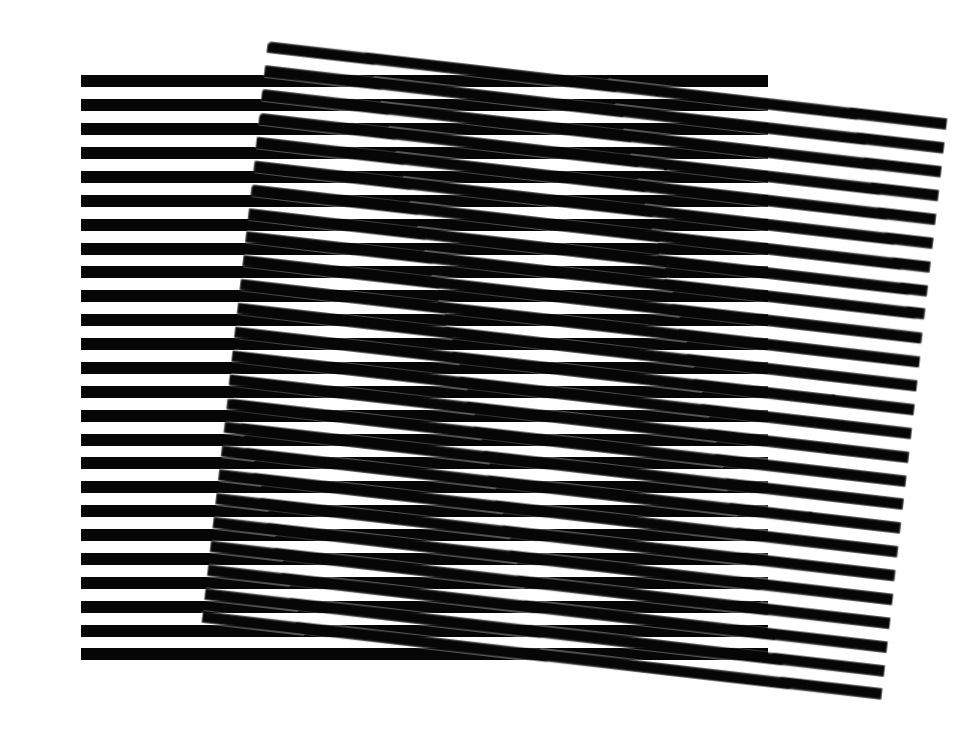
\includegraphics[scale=0.5]{figures/moire.png}
    \caption{Moir\'{e} Fringes}
    \label{fig:moire}
\end{figure}

In order to correctly interpret this interference effect, and reconstruct a super-resolved image,
multiple images need to be acquired from the microscope and analysed in the Fourier domain \cite{originalSIM}.
When reconstructed properly, there will be an improvement of lateral resolution in the direction of the k-vector of the pattern.
Therefore, when acquiring images for 2D SIM, it is almost always 3 groups of images that are acquired,
using patterns whose orientations are angled at multiples of $2\pi/3$ radians,
to obtain an near-isotropic improvement in \textit{lateral} resolution,
and the same is true in 3D SIM.
Within these groups, the images are acquired with the illumination pattern having a different phase each time,
typically with a constant offset between phases.

The reconstruction involves six key steps:

\begin{enumerate}
    \item parameter estimation,
    \item fourier transform,
    \item band separation,
    \item Wiener filtering,
    \item apodization, and,
    \item inverse Fourier transform.
\end{enumerate}

Parameter estimation is primarily concerned with the position of the illumination pattern,
including the phase, angle, and modulation depth.
This is more accurate than measuring these quantities in the physical system which would require a high degree of care and precision.
Then the image is converted to the frequency domain.

Denoting the image intensity by $D(\vec{r})$, the pattern k-vector and phase by $\vec{p}$, $\phi_n$,
the modulation depth by $a_m$, the density of the fluorescent substance as $S(\vec{r})$ and the point-spread function by $H(\vec{r})$,
we see that the effect of the optical system on the `true' ground-truth structure $S$ is to multiply it with the excitation pattern,
and then convolve with the point-spread function:

\[D_n(\vec{r}) = \sum_{m=-M}^{M}{S(\vec{r})a_m\exp(im(2\pi\vec{p}\cdot\vec{r}+\phi_n))\otimes H(\vec{r})}\]

Utilising the Convolution Theorem this becomes

\[\tilde{D}_n(\vec{k}) = \sum_{m=-M}^{M}{\exp(im\phi_n)a_m\tilde{S}(\vec{k}-m\vec{p})\tilde{O}(\vec{k})}\]

In turn, with sufficient acquired images at different phases, namely M, this can be used to solve a fully determined set of linear equations for

\[\tilde{S}(\vec{k}-m\vec{p})\tilde{O}(\vec{k})\qquad m=-M,\dots,M-1,M\]

This constitutes the band separation step, and explains why 2D SIM uses 3 sets of 3 images, while 3D SIM uses 3 sets of 5 images;
the number of different phases used in imaging must correspond to the number of delta peaks that represent the illumination pattern in Fourier space,
in order to set up a fully-determined system of linear equations \cite{params}.

The steps of Wiener filtering and apodization are used to combine the separated bands of the image, ...

The parameters used for the reconstructions are shown in Table \ref{tab:reconparams}

\begin{table}[htp]
    \centering
    \begin{tabular}{| c | c | c | c |}
        \hline
        Parameter & 2D Dataset (1) & 2D Dataset (2) & 3D Dataset \\
        \hline
        $\NA$  & 1.1 & 1.1 & 1.12 \\
        \hline
        Pixel width (nm) & 107 & 107 & 50 \\
        \hline
        Wavelength (nm) & 488 & 561 & 464 \\
        \hline
        OTF param.  & 0.15 & 0.15 & 0.15 \\
        \hline
        APO cutoff & 1.59 & 1.68 & 1.82 \\
        \hline
        APO bend  & 1.0 & 1.0 & 1.0 \\
        \hline
        Wiener parameter & 0.05 & 0.05 & 0.05 \\
        \hline
        RL Iterations & 5 & 5 & 5\\
        \hline

    \end{tabular}
    \caption{Parameters used to reconstruct the images in fairSIM.}
    \label{tab:reconparams}
\end{table}

\subsection{Data}

In the original work, Li et al. acquired pairs of high and low SNR images from a 3D SIM system,
in order to train the networks.
This project takes a slightly different approach,
simulating the increased image noise from a lower the illumination intensity in-silico.
This makes the acquisition of the training data much faster,
and avoids the need for image-pair registration, along with the errors that this could induce.
A low SNR image is simulated from the ground-truth high SNR image on a pixel-by-pixel basis:
a pixel whose value is $N$ in the high SNR image is set to a random draw of a Poisson random variable whose rate parameter is $N$/$s$,
where $s$ is some chosen scale factor constant across all pixels and images.
In both datasets this scale factor is set as 20.

The method is applied to a dataset of 2D SIM images in the first instance,
in which human cells are stained with AlexaFluor 488 and ATTO 565 fluorescent dyes.
These dyes illuminate the endoplasmic reticulum (ER) and microtubules, respectively.
This contains more high spatial frequency content that can be resolved by SIM than an earlier dataset acquired for the project,
in which viruses and the cell membrane of the host cell were highlighted.
The samples were illuminated with visible light at 488nm and 561nm.

\begin{figure}[hbtp]
    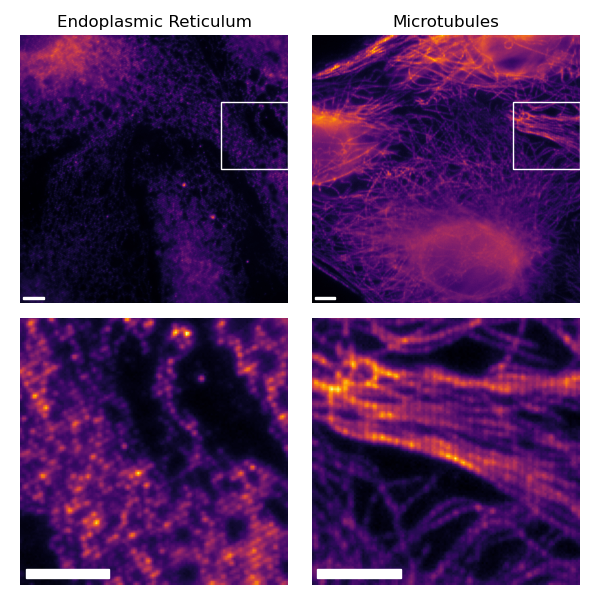
\includegraphics[scale=0.53, center]{figures/2DSIM.png}
    \caption{Images acquired from the physical 2DSIM system (one of a stack of 9).
    Top row: full 512x512 image. Bottom row: cropped region---the structured illumination pattern is visible.}
    \label{fig:2DSIM}
\end{figure}

In the second case, the Visible Human Dataset\footnote{Courtesy of the U.S. National Library of Medicine} is used to generate synthetically acquired 3DSIM micrographs.
This dataset was released in 1994 [cite] and provides images of human cadavers prepared as a series of thousands of thin cross sections.
The work uses the 70mm photographs of the female body dataset, image 2000 through to 2383.
While this imagery does not capture \textit{microscopic} biological structures,
those biological structures present are complex enough to yield an approximation to the image features one might expect from a typical SIM micrograph of a cell.
These images are downloaded, cropped into 256x256 squares 3 and stacked into image volumes of size (128, 256, 256).
Figure \ref{fig:vhcrop} shows the lateral cropping scheme overlayed onto image 2192,
the central image slice used.
The cropping is designed to produce 60 image volumes that mostly overlap with the biological subject matter,
for a total of 180 volumes when all 384 images are processed.

\begin{figure}[hbtp]
    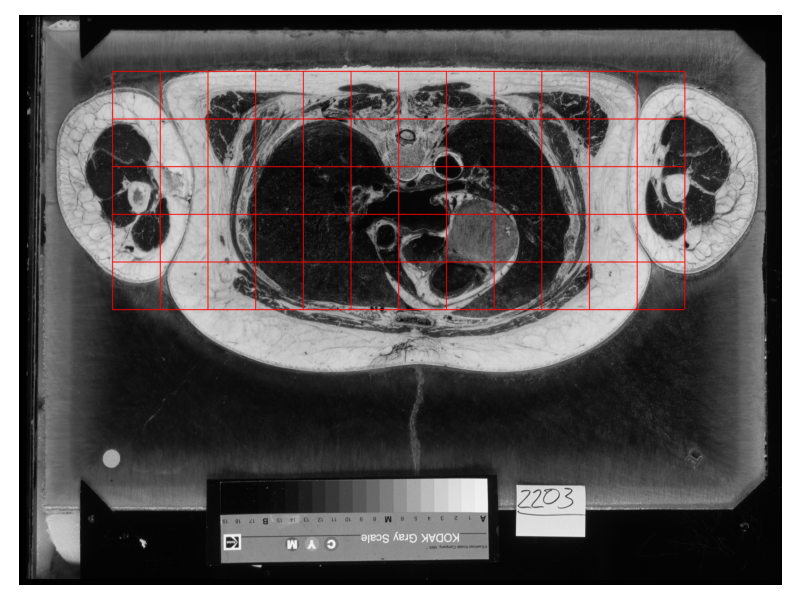
\includegraphics[scale=0.65, center]{figures/visible_human_volumes_grey.png}
    \caption{Cropping of Visible Human Dataset images}
    \label{fig:vhcrop}
\end{figure}

\begin{figure}[hbtp]
    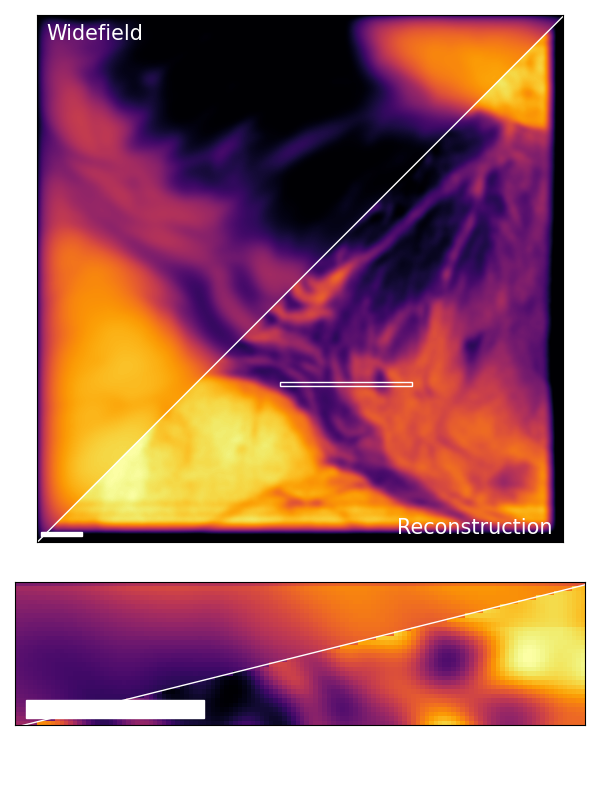
\includegraphics[scale=0.8, center]{figures/3DSIM_recon.png}
    \caption{Synthetic 3D SIM imagery. Top: central lateral cross-section. Bottom: Axial view from highlighted region. White bars are 1.0\textmu m wide.}
    \label{fig:3D_SIM}
\end{figure}

The volumes are then processed using \texttt{generate\_sim.py} to generate synthetic SIM acquisitions.
This script was adapted from [cite].
Originally, this script took an image volume of size (64, 256, 256) and generated an image stack of size (15, 256, 256),
simulating 15 SIM acquisitions from a microscope whose focal plane is at the central (32nd) slice of the 3D volume.
This was adapted further to simulate a 3D SIM microscope with a vertically moving objective lens and focal plane.
This effect was achieved by cropping the bottom $n$ lateral slices of the 3D volume and padding the top of the volume with $n$ zero-filled layers,
in order to move the focal plane to z-slice $32-n$ of the original volume.
A loop was used to generate a full (32, 15, 256, 256) 3DSIM acquisition stack,
equivalent to imaging the top half of the sample.
Each of the image volumes generated with a height of 128 voxels was used to generate two of these stacks.

[Diagram]

\subsection{Pipeline}

Migration to TensorFlow

The first step of the data processing pipeline is to produce the training-validation-testing partition,
which can be done using \texttt{image\_noising.py}.
This script takes a directory of high-SNR images, produces the synthetic low-SNR data counterpart images,
and then splits the data into training, validation, and testing partitions randomly.
In this work, 20\% of each dataset was reserved as testing data,
and a further 20\% of the remaining images were reserved for validation at the end of each epoch.

An RCAN model is then trained using this partitioned data - the `first-step' model.
This step is handled by the \texttt{train.py} script.
The code first reads in the configuration for training from a JSON file.
This file specifies:
\begin{itemize}
    \item training hyperparameters; such as number of epochs and the learning rate,
    \item model hyperparameters, and,
    \item file management; including the frequency of model checkpointing and the locations of training and validation data.
\end{itemize}
Configuring the hyperparameters in this way ensures that it is easier to keep track of the many training runs that may be performed.
Next, the training and validation data is read one file at a time, to perform checks---for instance to ensure that all of the images are of the same shape,
and that the data is consistent with model hyperparameters.
After this, the relevant training objects are instantiated: the model itself, the Adam optimizer, and the learning rate scheduler.
If an intermediate model checkpoint has been provided, all of these objects are updated to match the state of this checkpoint,
to enable continued training.
Alongside these is the \texttt{SIM\_Dataset} object wrapped in a \texttt{torch.utils.data.DataLoader} which handles the batching of training (and validation) data.

During training, this dataset object handles generation of suitable ground-truth and raw data.
Crucially, the RCAN input shape is smaller than the images themselves,
so the \texttt{SIM\_Dataset} takes random matching crops of the training pairs that correspond to the RCAN input shape.
It then normalises the pixel values, using an affine rescaling to map extreme image-wide pixel value percentiles to 0 and 1;
this work uses the values 2\% and 99.9\% respectively.
Before these crops are outputted, they are also subjected to a random 90 degree rotation about the z-axis,
and two random reflections in the lateral axes.
By employing these simple transformations for data augmentation,
we ensure that the very fine illumination structure signal is not degraded by, say, pixel value interpolation,
so that the reconstruction algorithm performance is unaffected.
This data augmentation increases the number of possible output crops by 16-fold,
on top of the number of possible crop locations.
Accordingly, the dataset object takes a \texttt{steps\_per\_epoch} parameter---this
parameter controls exactly how many times each image in the dataset is exposed to the training loop per epoch,
but with various different transformations.
In addition, the object is also able to filter for regions of interest.
The number of pixel values (scaled in the $[0, 1]$ range) that exceed some intensity threshold can be counted,
and then crops with an insufficient fraction of pixel values above this level can be excluded.
However, this slows down the speed of batch-loading, not just because of the rejection rate,
but also the computation required to run this check.

The model is then applied to the raw images.
In this step, the raw images undergo the same percentile-based standardisation as during training.
They are then inputted into the model, and the `restored' output is scaled to the full 16 bit-depth range and saved.
This leaves the ground-truth, raw, and restored SIM acquisition stacks,
which are pre-processed before reconstruction.
Specifically, each image has its acquisitions equalised so that they all have equal total pixel intensity.
We then perform a background subtraction of the lowest 10\% of pixel values, as well as clipping the brightest 0.1\% of pixel values.
In both cases the extreme values are masked at the threshold percentile intensities.
The data is then scaled to full 16 bit-depth range and saved.

The SIM reconstruction algorithm is then applied to the three sets of images.
For this purpose, fairSIM 1.4.1 \cite{fairSIM} was used.
While the original authors of the work provide their own software that can perform this reconstruction,
fairSIM presents a standard, open-source tool that is widely used for SIM image processing,
therefore making it worthwhile to investigate if the method is reproducible with this specific implementation of the reconstruction.
To this end, part of the codebase is dedicated to enabling compatibility with the fairSIM application.
Namely, the scripts:
\begin{itemize}
    \item \texttt{convert\_omx\_to\_czxy.py},
    \item \texttt{convert\_omx\_to\_paz.py}, and,
    \item \texttt{manage\_stack.py},
\end{itemize}
can be used to convert between CZXY format (used for model training) and the OMX and PAZ formats.
This is particularly useful in the case of 3D image reconstructions which take much longer,
since in our case 32 reconstructions have to be performed per image.
Converting to PAZ and then stacking the SIM acquisition stacks enables the fairSIM `batch' feature to be used,
to automate the reconstruction of the entire stack.
This means that the only limit is the size of image volume that can be loaded into fairSIM.

Once the reconstructions are performed they are destacked, if necessary, and postprocessed to clip negative values that arise in the SIM reconstruction,
and again scaled to the full 16 bit-depth range and saved.

At this point the `first-step' reconstructions, those from the restored acquisition stacks,
can be compared to the reconstructions from the low and high SNR data.
Additionally, the training data for the second-step denoising model can be collated.
This second model takes the restored reconstructions as its input, and the high SNR reconstructions as its target.
After training, the model is applied to the testing high SNR reconstructions, and post processed in the same way as previously.

This pipeline was developed with software best practices in mind.


Software best practices
I/O, documentation, modularity, version control

Using CSD3, hardware, parallel -> serial.
Estimates of the duration for the entire pipeline.

\subsection{RCAN}

In both instances, the denoising models were implemented using the residual channel attention network (RCAN) architecture,
which first emerged in the computer vision literature in 2018 \cite{rcan2018}.
The fundamental component of this architecture is the `channel attention layer'.
This unit:

\begin{itemize}
    \item summarises the features extracted in each hidden channel using a global pooling operation,
    \item computes `attention weights' for each channel via a simple mechanism;
    namely downsample the number of channels using a 1x1 convolution,
    apply ReLU activation,
    upsample to the number of original channels via 1x1 convolution,
    and apply sigmoid activation, and,
    \item multiple each channel from the input to the layer by the computed attention weights.
\end{itemize}

This is a fairly rudimentary form of attention mechanism compared to more sophisticated transformer models.
However, the RCAN builds on this elementary component by combining multiple channel attention layers (or blocks) into 'residual groups'.
A single group consists of a series of 3x3 convolution layers to extract features,
followed by a channel attention layer, together with a residual connection in which the input is added.
Many of these layer sequences are chained together to form a single residual group.
Moreover, an RCAN itself consists of multiple residual groups chained together,
with intermediate residual connections as well as a `long' skip connection which spans the entire network length.
This complex residual structure of the network implements a model which, theoretically, is very deep.

Li et al. employed a slight variant of the RCAN implemented more recently \cite{rcan2021}.
In particular, this variant is re-implemented as a denoising model rather than a super-resolution model,
so there is no upsampling of the images over the course of the network architecture.
However, the code provided alongside this more recent work is written in TensorFlow.
In order to make the code compatible with the software available (specifically the versions of CUDA and cuDNN available) on the HPC platform used,
this codebase was migrated to PyTorch.
This also has the advantage of making the software more accessible to other researchers wishing to develop in PyTorch.

\section{Results}

Affine rescaling to minimize the MSE to the GT?
Discuss the results they found

\subsection{2D Data}

The 2D image processing pipeline uses RCAN models taking a 128x128 input region,
and with an architecture comprising 5 residual groups of 3 blocks each.
During image denoising, the input image is patched into regions having a 32 pixel overlap,
and the model is applied to each region independently.
The predictions are then averaged in regions of the image where patches overlap,
avoiding the creation of edge artefacts at the borders of the patching regime.

\begin{figure}[hbtp]
    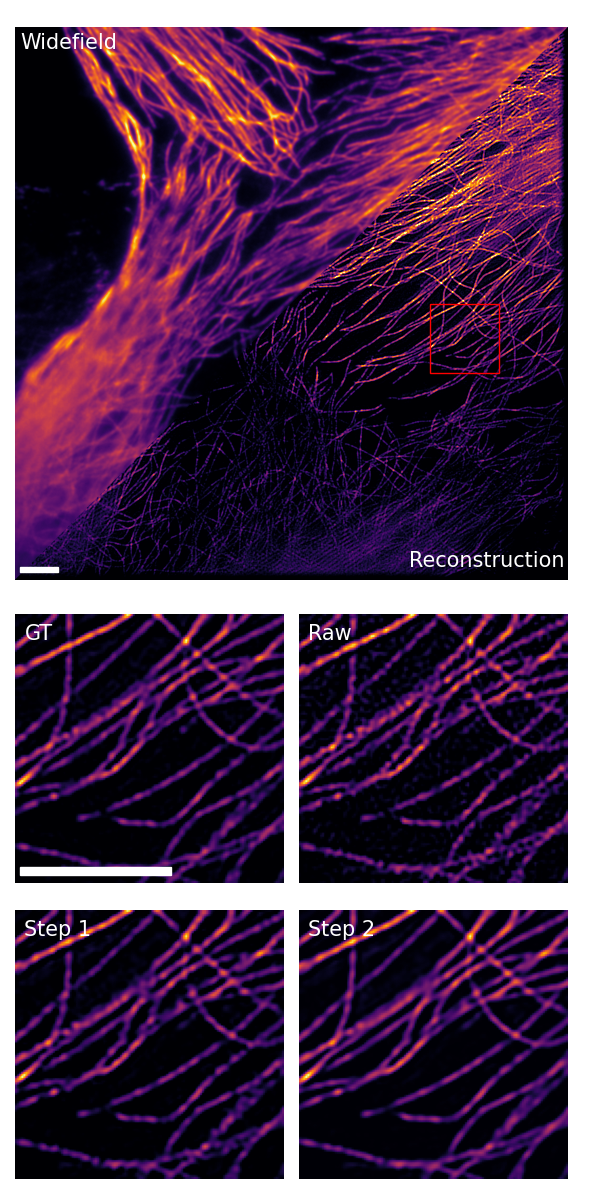
\includegraphics[scale=0.8, center]{figures/microtub_samples.png}
    \caption{A 2D SIM microtubules image showing the steps of the model pipeline.
    Top: Full ground-truth (GT) image. Bottom: Reconstructions from high SNR, low SNR, and restored images. White rectangles are 3.9\textmu m wide.}
    \label{fig:microtub_samples}
\end{figure}

\begin{figure}[hbtp]
    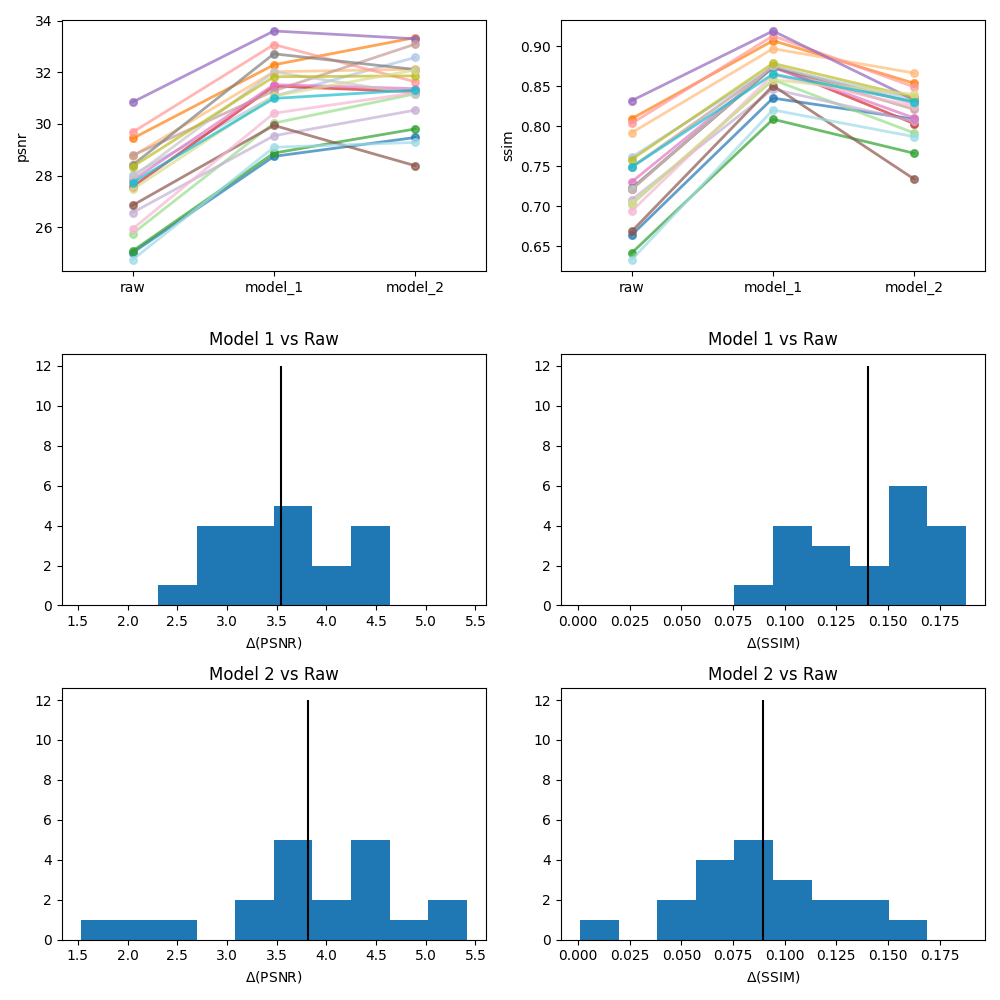
\includegraphics[scale=0.7, center]{figures/m019_m020_pipeline_stats.png}
    \caption{Performance of pipeline trained to reconstruct microtubule images, evaluated on the test dataset of size 20.
    In the histograms the black line indicates the mean metric change}
    \label{fig:m019_m020_pipeline_stats}
\end{figure}

Initially, only the microtubule images were used for model training.
Both models were trained for 500 epochs.
Figure \ref{fig:microtub_samples} shows an example of the denoising pipeline applied to an image from the test dataset.
In the `Raw' reconstruction we can see the ringing artefacts created by the increased noise in the SIM acquisitions used.
The bottom left reconstruction was achieved by denoising the low SNR acquisition before applying the reconstruction,
while in the bottom right, this reconstruction was passed through the further second model.
In both of the pipeline reconstructions, we observe a removal of the ringing artefacts present in the low SNR reconstruction.

Figure \ref{fig:m019_m020_pipeline_stats} shows the results of applying this pipeline to the test data.
The complete two-step reconstructions have a peak signal-to-noise ratio (PSNR) with reference to the ground-truth reconstructions which is on average 3.8 dB higher than the low SNR reconstructions.
Similarly the structural simimlarity index measure (SSIM) improves by 0.09 on average.
These improvements correspond to a qualitative improvement in the reconstruction in Figure \ref{fig:microtub_samples}.
However, most of this improvement can be attributed to the first-step model.
Indeed, the reconstruction does not appear to change much visually after the second step denoising,
and in fact the SSIM of the reconstruction decreases by 0.05 on average after the second step is applied.
Additionally the first-step reconstructions appear to be more consistent in their quantitative improvements than the full two-step restoration.

\begin{figure}[hbtp]
    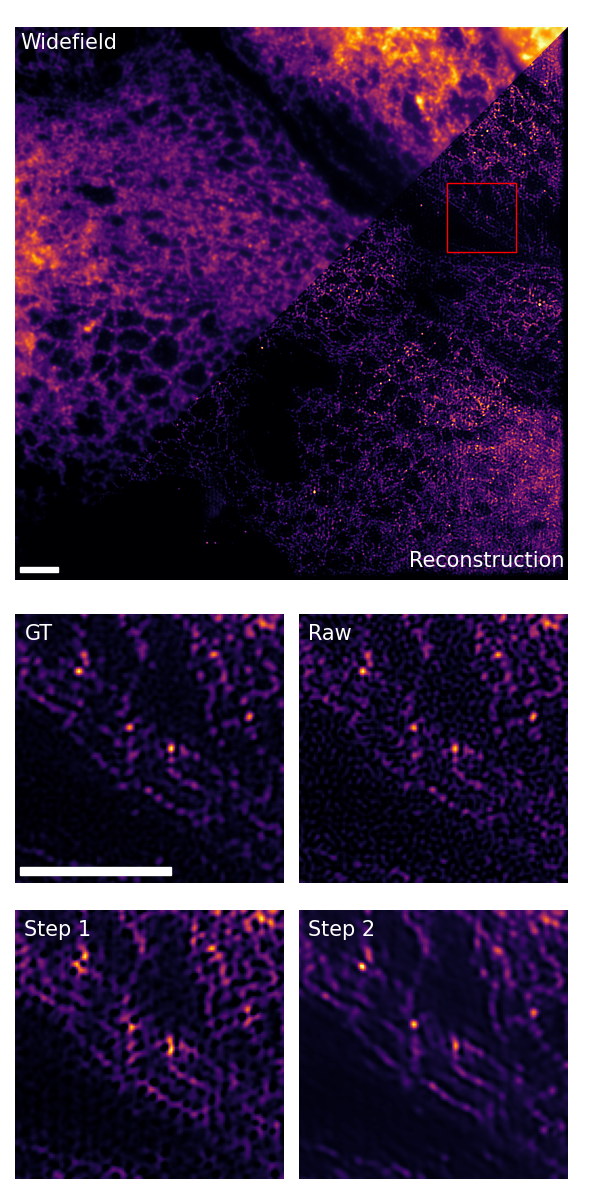
\includegraphics[scale=0.78, center]{figures/er_samples.png}
    \caption{Sample of the results from the 2D SIM restoration applied to both fluorescence channels.
    Top: Full ground-truth (GT) image. Bottom: Reconstructions from high SNR, low SNR, and restored images. White rectangles are 3.9\textmu m wide.}
    \label{fig:er_samples}
\end{figure}

\begin{figure}[hbtp]
    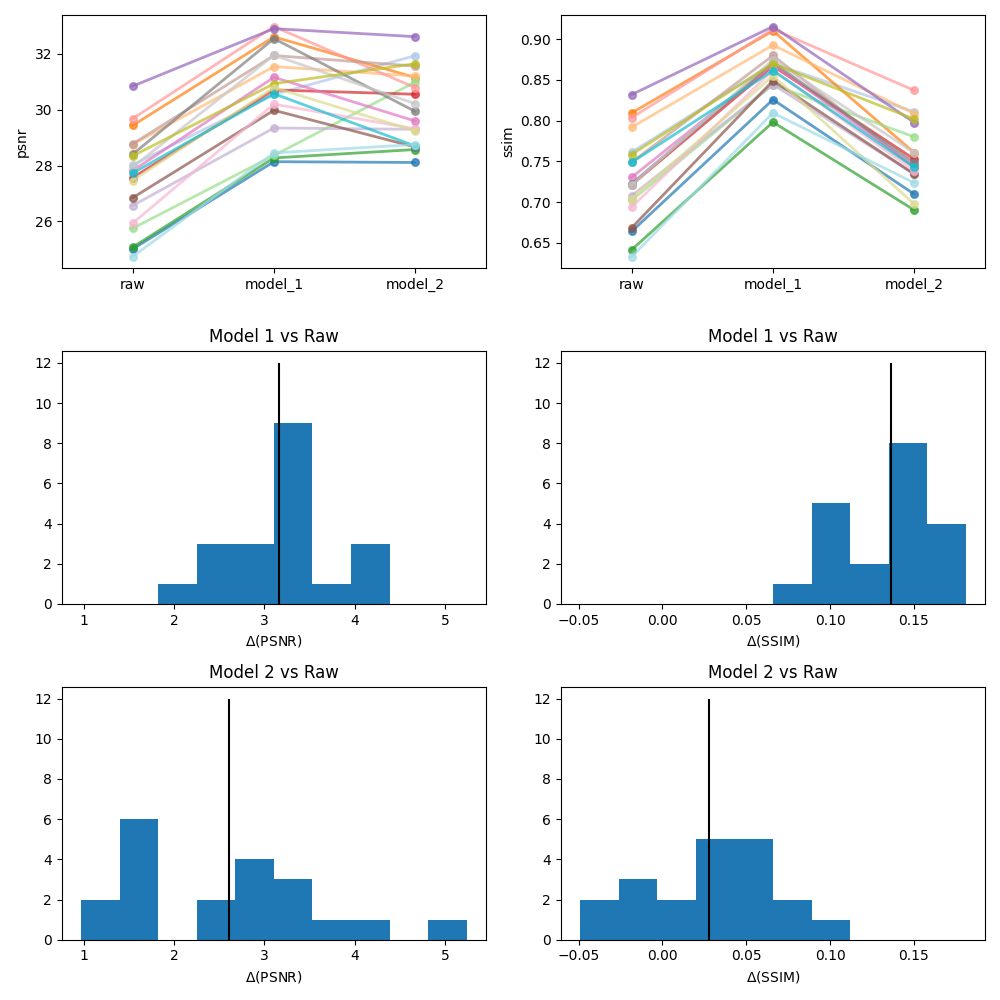
\includegraphics[scale=0.7, center]{figures/m023_m024_561_pipeline_stats.png}
    \caption{Performance of pipeline trained to reconstruct \textbf{microtubule} images, evaluated on the test dataset of size 20.
    In the histograms the black line indicates the mean metric change.}
    \label{fig:m023_m024_561_pipeline_stats}
\end{figure}

\begin{figure}[hbtp]
    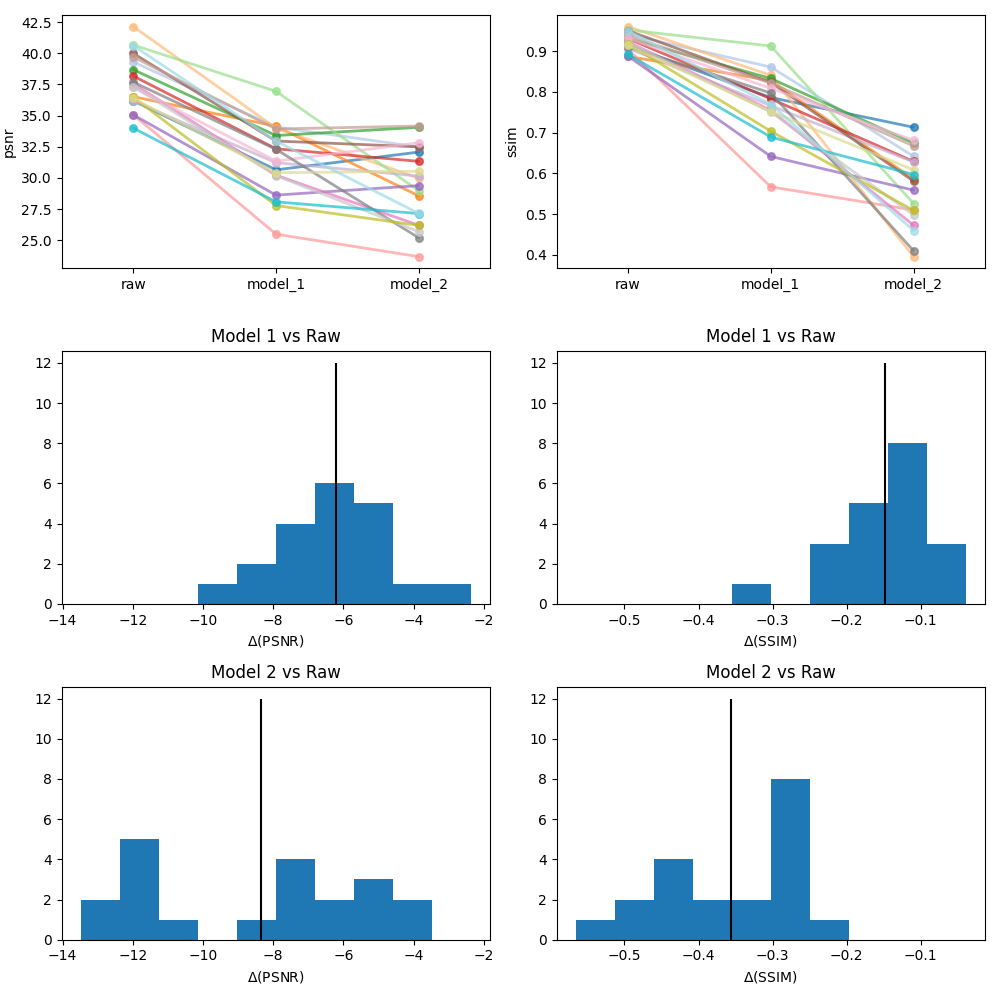
\includegraphics[scale=0.7, center]{figures/m023_m024_488_pipeline_stats.png}
    \caption{Performance of pipeline trained to reconstruct \textbf{ER} images, evaluated on the test dataset of size 20.
    In the histograms the black line indicates the mean metric change.}
    \label{fig:m023_m024_488_pipeline_stats}
\end{figure}

In the second instance, a pipeline with the same model hyperparameters was developed using the full dataset for model training:
both the ER and microtubule images.
The first model was trained for 245 epochs and the second for 500 epochs.
The results of this model as applied to an ER test image is shown in Figure \ref{fig:er_samples}.
As before, the low SNR reconstruction contains ringing artefacts,
however in this case rather than being removed outright in the first-step reconstruction,
these are replaced by a different set of patterned artefacts.
The full two-step reconstruction manages to mitigate these new artefacts,
although it is concerning that some of the rough textures of the ground-truth reconstruction appear to be lost in the second step.
This raises the possibility that in the denoising process,
it may be difficult for the model to discriminate between true fine features and artificial ones introduced by noise.
The inspection of restoration performance in Figure \ref{fig:er_samples} is reflected in Figure \ref{fig:m023_m024_488_pipeline_stats},
where the quantitative evaluation of both steps of this model decreases in terms of both PSNR and SSIM, for ER images.
It is worth noting that the fidelity of the raw ER images is higher on average than for the microtubules,
however even in absolute terms, both the first-step and two-step denoised images perform much worse than the previous restoration pipeline in terms of the SSIM metric.
Additionally, increasing the diversity of training data also worsens the performance on the microtubules images;
the two-step form of this model only provided an increase of 2.6dB in PSNR and 0.03 for SSIM,
and a similar observation is true for the first-step restoration.

Ideas: apply the first model to (a) the ER images and
(b) the ER images but degraded even more so that their raw reconstructions are equivalent fidelity to the raw microtubule fidelity.
learning curves
SIM check results / Pattern estimation


\subsection{3D Data}

For the 3D data, the same training hyperparameters were used, except for the architecture.
Slightly larger RCAN models with 5 residual groups of 5 blocks each were used---matching the architecture employed by Li et al.
The first step model was trained for 41 epochs, the second for 24.
Figure \ref{fig:vh_samples_prong} demonstrates this reconstruction.
The low SNR reconstruction is consistent with the low SNR reconstruction from the 2D data,
suffering from irregular ringing artefacts.
As before, the first-step reconstruction removes these artefacts,
but appears to introduce new patterned artefacts.
In the Figure this pattern appears to take the form of a regular triangular lattice
---this was found to be common around the edges of high intensity regions.
Similarly, the axial views of the first-step reconstructions appear to be affected by regular patterned artefacts in the form of vertical `stripes',
this is more visible in some of the images in [appendix ref].
The full two-step restoration mitigates these artefacts in both the lateral and axial planes,
but appears again to be indiscriminate between features resulting from ground truth stuctures and those resulting from noise.
The skeleton in the lateral views of Figure \ref{fig:vh_samples_prong} demonstrates that this second-step is capable of morphing the true image structures:
in this case the three `needle' structures of the ground-truth image (which are preserved in the raw and first-step reconstructions) are moved and shortened.


PSNR / SSIM vs qualitative inspection (put stuff into appendix);

\begin{figure}[hbtp]
    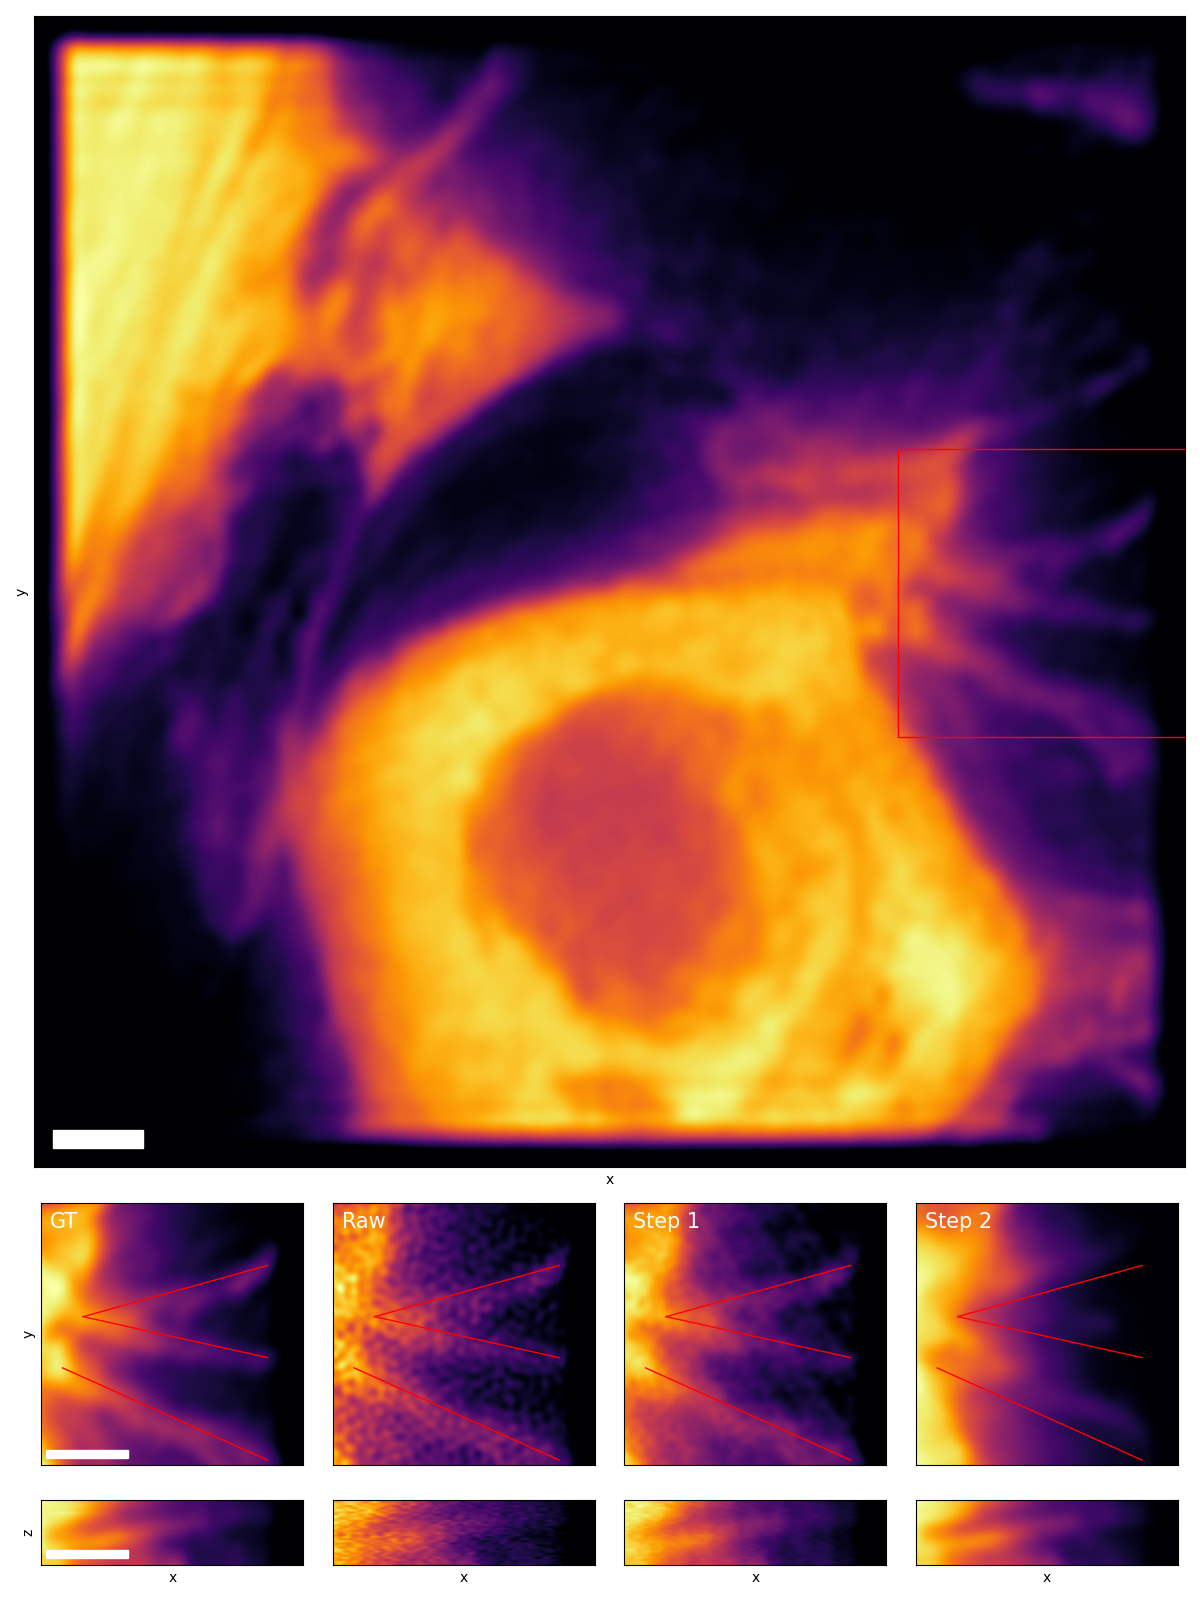
\includegraphics[scale=0.55, center]{figures/vh_samples_prong.png}
    \caption{Sample of the results from the 3D SIM restoration pipeline.
    Top: Full ground-truth (GT) image. Bottom: Lateral (above) and axial (below) views of reconstructions.
    Red skeleton superimposed onto lateral views is fixed. White rectangles are 1.0\textmu m wide.}
    \label{fig:vh_samples_prong}
\end{figure}

\begin{figure}[hbtp]
    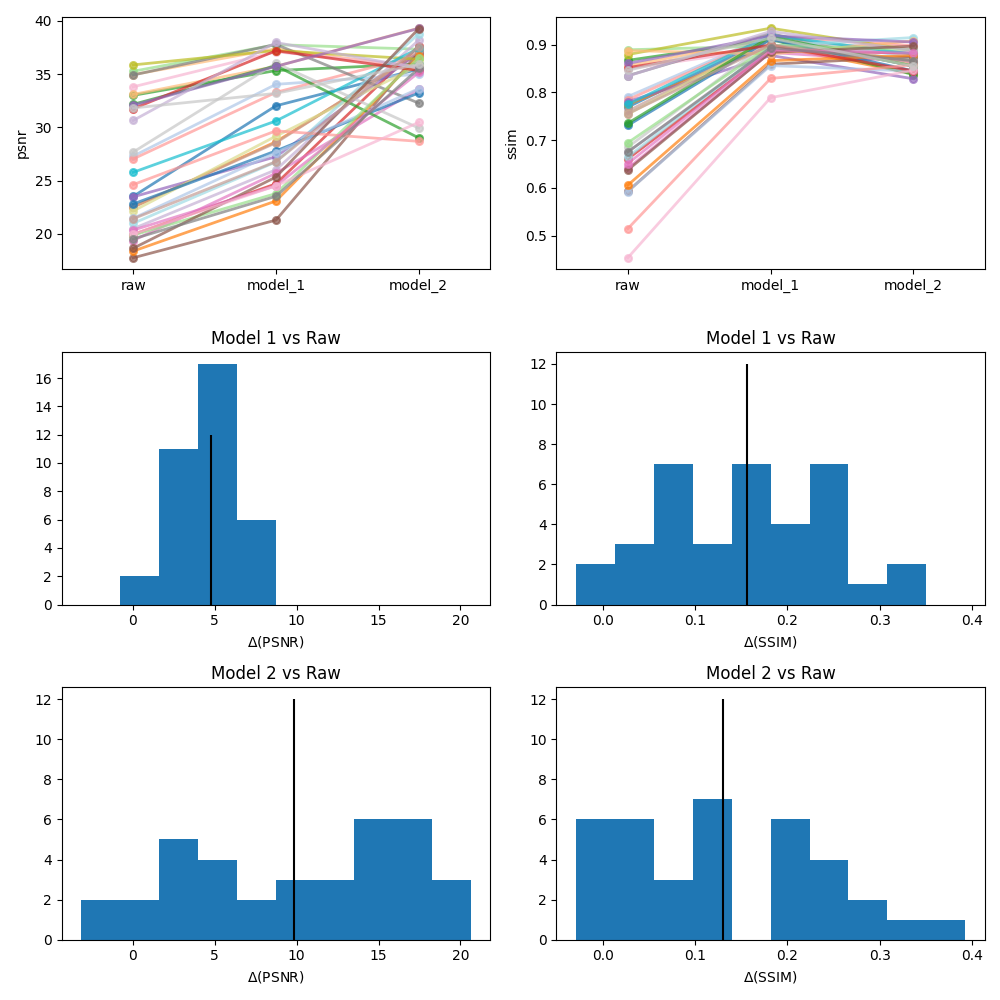
\includegraphics[scale=0.55, center]{figures/m021_m022_pipeline_stats.png}
    \caption{Performance of pipeline trained to reconstruct Visible Human images, evaluated on the test dataset of size 36.
    In the histograms the black line indicates the mean metric change.}
    \label{fig:vh_stats}
\end{figure}

Figure \ref{fig:vh_stats} shows the quantitative performance of the 3DSIM restorations.
According to both PSNR and SSIM, the 3DSIM restoration improves the data fidelity of the low SNR images quite considerably.
The two-step reconstructions lead to a 9.8\textpm 1.1 dB increase in PSNR in total,
with the first denoising step contributing 4.8\textpm 0.3 dB.
Similarly the SSIM improves by 0.13\textpm 0.02 as a result of the full two-step restoration,
although in this case the second step appears to slightly degrade the first-step reconstruction.


For comparison, the original research said 3.63 \textpm 1.31 dB and 0.15\textpm 0.09 (overestimates for the errors as we don't know correlation of psnr results between pairs)




Train-test-split resolve

Axial resolution

Removal of true structures. Adding the fact that the GT in this data had zero simulated microscope noise (Gaussian, Poisson)

Tables of results, metrics

Images

The fact that 2nd step improves in the 3D case may indicate that it is important to use separate train/val/splits



\section{Discussion}

This project investigated the reproducibility of the original research by Li et al. by applying the method they developed to multiple new datasets.
The sets of data used here represent different domains of images,
firstly because of the different ground-truth structures---ER and Visible Human imagery---and secondly
by using images acquired by SIM systems with slightly different specifications.
In particular the real images were acquired from a 2D SIM system rather than a 3D SIM system,
and even the 3D imagery was acquired from an optical system simulated in silico.
In the same vein, the reconstructions were performed using a more widespread tool, fairSIM,
rather than the bespoke reconstruction code used in the project,
in order to investigate whether the specific reconstruction algorithm might affect the performance of the method.
The work corroborated multiple claims that they made about the two-step RCAN method.
Indeed, this project demonstrated that the method is capable of removing ringing artefacts that result from reconstructing a stack of SIM images acquired at a low illumination intensity.
Although the first-step model can introduce new, patterned artefacts, these are typically mitigated by the further second step,
and this is made clear in Figure 5c in the paper \cite{keypaper}.
Moreover, the method produced statistically significant quantitative (?explain) improvements in the fidelity of the reconstructions,
according to both the PSNR and SSIM metrics, for the microtubule-only pipeline and the Visible Human denoising pipeline.

The work also uncovered some underlying issues with the model.
Primarily,

Some issues that were found
- The morphing of true structures by the second step.
- Separate train/test/val sets needed, further reducing amount of training data
- time taken to train
- issues with pattern estimation; find a reference on how ML can disturb this.

Further work
- Ideas from section 3 of image analysis
- Further training (learning curve, appendix)

Some things I could improve on, what I learned
- Augmentation: randomly permute the acquisitions?
    Bug: flipping the acquisition stack order
    No simulated noise in the 3D SIM GT
    Better poisson noising that is even across images
    Doing 2D SIM first was a good idea (breaking the problem down)

\bibliographystyle{IEEEtran}
\bibliography{Biblio}

\appendix

\section{Statement on the use of auto-generation tools}

\section {High-Performance Computing Resources}

This work was performed using resources provided by the Cambridge Service for Data Driven Discovery (CSD3) operated by the University of Cambridge Research Computing Service (www.csd3.cam.ac.uk),
provided by Dell EMC and Intel using Tier-2 funding from the Engineering and Physical Sciences Research Council (capital grant EP/T022159/1),
and DiRAC funding from the Science and Technology Facilities Council (www.dirac.ac.uk).

\end{document}
